%
% This is the LaTeX template file for lecture notes for EE 382C/EE 361C.
%
% To familiarize yourself with this template, the body contains
% some examples of its use.  Look them over.  Then you can
% run LaTeX on this file.  After you have LaTeXed this file then
% you can look over the result either by printing it out with
% dvips or using xdvi.
%
% This template is based on the template for Prof. Sinclair's CS 270.

\documentclass[twoside]{article}
\usepackage{graphics}
\usepackage{graphicx}
\usepackage{algorithm}
\usepackage{mathtools}
\usepackage{mathptmx}
\usepackage{algpseudocode}
\setlength{\oddsidemargin}{0.25 in}
\setlength{\evensidemargin}{-0.25 in}
\setlength{\topmargin}{-0.6 in}
\setlength{\textwidth}{6.5 in}
\setlength{\textheight}{8.5 in}
\setlength{\headsep}{0.75 in}
\setlength{\parindent}{0 in}
\setlength{\parskip}{0.1 in}

%
% The following commands set up the lecnum (lecture number)
% counter and make various numbering schemes work relative
% to the lecture number.
%
\newcounter{lecnum}
\renewcommand{\thepage}{\thelecnum-\arabic{page}}
\renewcommand{\thesection}{\thelecnum.\arabic{section}}
\renewcommand{\theequation}{\thelecnum.\arabic{equation}}
\renewcommand{\thefigure}{\thelecnum.\arabic{figure}}
\renewcommand{\thetable}{\thelecnum.\arabic{table}}

%
% The following macro is used to generate the header.
%
\newcommand{\lecture}[4]{
   \pagestyle{myheadings}
   \thispagestyle{plain}
   \newpage
   \setcounter{lecnum}{#1}
   \setcounter{page}{1}
   \noindent
   \begin{center}
   \framebox{
      \vbox{\vspace{2mm}
    \hbox to 6.28in { {\bf EE 382C/361C: Multicore Computing
                        \hfill Fall 2016} }
       \vspace{4mm}
       \hbox to 6.28in { {\Large \hfill Lecture #1: #2  \hfill} }
       \vspace{2mm}
       \hbox to 6.28in { {\it Lecturer: #3 \hfill Scribe: #4} }
      \vspace{2mm}}
   }
   \end{center}
   \markboth{Lecture #1: #2}{Lecture #1: #2}
   %{\bf Disclaimer}: {\it These notes have not been subjected to the
   %usual scrutiny reserved for formal publications.  They may be distributed
   %outside this class only with the permission of the Instructor.}
   \vspace*{4mm}
}

%
% Convention for citations is authors' initials followed by the year.
% For example, to cite a paper by Leighton and Maggs you would type
% \cite{LM89}, and to cite a paper by Strassen you would type \cite{S69}.
% (To avoid bibliography problems, for now we redefine the \cite command.)
% Also commands that create a suitable format for the reference list.
\renewcommand{\cite}[1]{[#1]}
\def\beginrefs{\begin{list}%
        {[\arabic{equation}]}{\usecounter{equation}
         \setlength{\leftmargin}{2.0truecm}\setlength{\labelsep}{0.4truecm}%
         \setlength{\labelwidth}{1.6truecm}}}
\def\endrefs{\end{list}}
\def\bibentry#1{\item[\hbox{[#1]}]}

%Use this command for a figure; it puts a figure in wherever you want it.
%usage: \fig{NUMBER}{SPACE-IN-INCHES}{CAPTION}
\newcommand{\fig}[3]{
			\vspace{#2}
			\begin{center}
			Figure \thelecnum.#1:~#3
			\end{center}
	}
% Use these for theorems, lemmas, proofs, etc.
\newtheorem{theorem}{Theorem}[lecnum]
\newtheorem{lemma}[theorem]{Lemma}
\newtheorem{proposition}[theorem]{Proposition}
\newtheorem{claim}[theorem]{Claim}
\newtheorem{corollary}[theorem]{Corollary}
\newtheorem{definition}[theorem]{Definition}
\newenvironment{proof}{{\bf Proof:}}{\hfill\rule{2mm}{2mm}}

% **** IF YOU WANT TO DEFINE ADDITIONAL MACROS FOR YOURSELF, PUT THEM HERE:

\begin{document}
%FILL IN THE RIGHT INFO.
%\lecture{**LECTURE-NUMBER**}{**DATE**}{**LECTURER**}{**SCRIBE**}
\lecture{8}{September 20}{Vijay Garg}{Liheng Ding}
%\footnotetext{These notes are partially based on those of Nigel Mansell.}

% **** YOUR NOTES GO HERE:

% Some general latex examples and examples making use of the
% macros follow.  
%**** IN GENERAL, BE BRIEF. LONG SCRIBE NOTES, NO MATTER HOW WELL WRITTEN,
%**** ARE NEVER READ BY ANYBODY.
\section{Introduction}
%Students in EE 382C are required to scribe lecture notes for one lecture.
%These lecture notes will be done using the document processing system called Latex.
%We have posted the file {\em scribe.tex} on the Canvas system. You can run {\tt pdflatex}
%on that file to generate {\em scribe.pdf}. The remaining document shows usage of
%some of the commands in Latex.
\indent This lecture covers following topics:
\begin{enumerate}
	\item Locks with Get-and-Set Operation
	\item Queue Locks
\end{enumerate}

\section{Locks with Get-and-Set Operation}
Although locks for mutual exclusion can be built using simple read and write instructions, any such algorithm requires as many memory locations as the number of threads. By using instructions with higher atomicity, it is much easier to build locks. For example, the \textit{getAndSet} operation (also called \textit{testAndSet}) allows us to build a lock as shown in Alogrithm
\ref{alg:getandset}.

\begin{algorithm}
\caption{Building Locks Using GetAndSet.}
\begin{algorithmic}[1]
\State import java.util.concurrent.atomic.*;
\State public class GetAndSet implements MyLock \{
\State \indent AtomicBoolean isOccupied = new AtomicBoolean(false);
\State \indent public void lock() \{
\State \indent \indent while (isOccupied.getAndSet(true))
\State \indent \indent \indent Thread.yield(); 
\State \indent \indent \indent \text{// skip();}
\State \indent \indent \} 
\State \indent \}
\State \indent public void unlock() \{
\State \indent \indent isOccupied.set(false);
\State \indent \}
\State \}
\end{algorithmic}
\label{alg:getandset}
\end{algorithm}

This algorithm satisfies the mutual exclusion and progress property. However, it does not satisfy starvation freedom.
Besides, keeping invoking \textit{getAndSet} is not efficient enough since this method will use a shared bus to get access to \textit{isOccupied}. So an alternative implementation is shown in Algorithm \ref{alg:getandgetandset}.

\begin{algorithm}
\caption{Building Locks Using GetAndGetAndSet.}
\begin{algorithmic}[1]
\State import java.util.concurrent.atomic.*;
\State public class GetAndGetAndSet implements MyLock \{
\State \indent AtomicBoolean isOccupied = new AtomicBoolean(false);
\State \indent public void lock() \{
\State \indent \indent while (true)\{
\State \indent \indent \indent while (isOccupied.get()) \{
\State \indent \indent \indent \}
\State \indent \indent \indent if (! isOccupied.getAndSet(true)) return;
\State \indent \indent \} 
\State \indent \}
\State \indent public void unlock() \{
\State \indent \indent isOccupied.set(false);
\State \indent \}
\State \}
\end{algorithmic}
\label{alg:getandgetandset}
\end{algorithm}

In this implementation, a thread first checks if the lock is available using the \textit{get} operation. It calls the \textit{getAndSet} operation only when it finds the critical section available. If it succeeds in \textit{getAndSet}, then it enters the critical section; otherwise, it goes back to spinning on the \textit{get} operation.

However, high bus contention still happens when all threads get that \textit{isOccupied.get()} is \textit{false} and try to set it to \textit{true} by using \textit{getAndSet()}. So a better implementation using \textit{Backoff} is shown in Algorithm \ref{alg:backoff}. The thread fails to set \textit{getAndSet()} will back off for a certain period of time. 

\begin{algorithm}
\caption{Building Locks Using Backoff.}
\begin{algorithmic}[1]
\State import java.util.concurrent.atomic.*;
\State public class GetAndGetAndSet implements MyLock \{
\State \indent AtomicBoolean isOccupied = new AtomicBoolean(false);
\State \indent public void lock() \{
\State \indent \indent while (true)\{
\State \indent \indent \indent while (isOccupied.get()) \{
\State \indent \indent \indent \}
\State \indent \indent \indent if (! isOccupied.getAndSet(true)) return;
\State \indent \indent \indent else \{
\State \indent \indent \indent \indent int timeToSleep = calculateDuration();
\State \indent \indent \indent \indent Thread.sleep(timeToSleep);
\State \indent \indent \indent \}
\State \indent \indent \} 
\State \indent \}
\State \indent public void unlock() \{
\State \indent \indent isOccupied.set(false);
\State \indent \}
\State \}
\end{algorithmic}
\label{alg:backoff}
\end{algorithm}


\section{Queue Locks}
Previous approaches to solve mutual exclusion require threads to spin on the shared memory location. In this section, we present alternate methods to avoid spinning on the same memory location. All methods maintain a queue of threads waiting to enter the critical section. Anderson's lock uses a fixed size array, CLH lock uses an implicit linked list and MCS lock uses an explicit linked list for the queue. One of the key challenges in designing these algorithms is that we cannot use locks to update the queue.

\subsection{Anderson's Lock}
Anderson's lock uses a circular array \textbf{Available} of size \emph{n} which is at least as big as the number of threads that may be contending for the critical section. The array is circular so that the index \emph{i} in the array is always a value in the range 0..$n-1$ and is incremented modulo \emph{n}. Different threads waiting for the critical section spin on the different slots in this array thus avoiding the problem of multiple threads spinning on the same variable. 

\begin{figure}[ht]
  \centering
  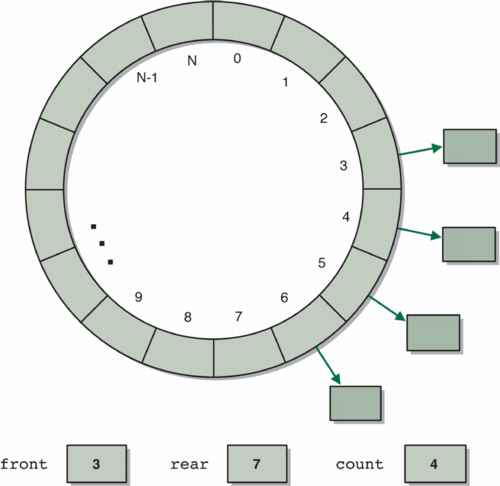
\includegraphics[height=0.38\textheight,width=0.5\linewidth]{./CircularArray.png} 
  \caption{Circular Array}
  \label{fig:ql}
\end{figure}

Note that the above description assumes that each slot is big enough so that adjacent slots do not share a cache line. Hence even though we just need a single bit to store \textbf{Available[i]}, it is important to keep it big enough by padding to avoid the problem of \textit{false sharing}. Also note that since Anderson's lock assigns slots to threads in the FCFS manner, it guarantees fairness and therefore freedom from starvation.

A problem with Anderson lock is that it requires a separate array of size \emph{n} for each lock. Hence, a system that uses \emph{m} locks shared among \emph{n} threads will use up \emph{O(nm)} space.

\begin{algorithm}
\caption{pseudo code for Anderson Lock}
\begin{algorithmic}[1]
\State public class AndersonLock \{
\State \indent AtomicInteger tailSlot = new AtomicInteger (0); 
\State \indent boolean [ ] Avaliable ;
\State \indent ThreadLocal \textless Integer\textgreater mySlot; \text{// initialize to 0} \newline
\State \indent public AndersonLock (int n) \{ \text{// constructor}
\State \indent \} \text{// all Available false except Available[0]}
\State \indent public void lock() \{
\State \indent \indent mySlot.set(tailSlot.getAndIncrement() \% n);
\State \indent \indent spinUntil (Available[mySlot]);
\State \indent \}
\State \indent public void unlock() \{
\State \indent \indent Available[mySlot.get()] = false;
\State \indent \indent Available[(mySlot.get()+1) \% n] = true;
\State \indent \}
\State \}
\end{algorithmic}
\label{alg:anderson}
\end{algorithm}

\subsection{CLH Queue Lock}


We can reduce the memory consumption in Anderson's algorithm by using a dynamic linked list instead of a fixed size array. Any thread that wants to get lock inserts a node in the linked list. The insertion in the linked list must be atomic. The sub-algorithm is shown in Algorithm \ref{alg:clh} and full algorithm can be found at \cite{1}. It is important to note that if the thread exists the CS wants to enter the CS again, it cannot reuse its own node because the next thread may still spinning on that node's field. Therefore, it uses the predecessor in the \textit{unlock} function.

The linked list is virtual. The thread that is spinning has the variable \textit{pred} that points to the predecessor node in the linked list.

\begin{algorithm}
\caption{pseudo code for CLH Queue Lock}
\begin{algorithmic}[1]
\State class Node \{
\State \indent boolean locked;
\State \}
\State AtomicReference\textless Node\textgreater tailNode;
\State ThreadLocal\textless Node\textgreater myNode;
\State ThreadLocal\textless Node\textgreater pred;
\State lock() \{
\State \indent myNode.locked = true;
\State \indent pred = tailNode.getAndSet(myNode);
\State \indent while(pred.locked) \{ noops; \}
\State \}
\State unlock() \{
\State \indent myNode.locked = false;
\State \indent myNode = pred; \text{// reuse pred node for future}
\State \}
\end{algorithmic}
\label{alg:clh}
\end{algorithm}

\subsection{MCS Queue Lock}

In many architectures, each core may have local memory such that access to its local memory is fast but access to the local memory of another core is slower. In such architectures, CLH algorithm results in threads spinning on remote locations. MCS avoids the remote spinning. Same as CLH, MCS maintain a queue. However, it is an explicit linked list. 

The tricky part of MCS is in the \textit{unlock()} function. When a thread \textit{p} exits the CS, it checks if there is any node linked next to its node. If there exits such node, then it makes the \textit{locked} false and removes its node from the linked list. When it finds no node linked next to it, there can be two cases for this. First, no thread has been inserted yet. Therefore, we can find that \textit{tailNode} still points to \textit{myNode}. It can be simply reset to null. In the second case, thread \textit{p} waits until the next is not null. Then it can set the locked field for that node to be false as usual. This is shown in Algorithm \ref{alg:mcs}.

\begin{algorithm}
\caption{pseudo code for MCS Queue Lock}
\begin{algorithmic}[1]
\State class QNode \{
\State \indent boolean locked; \text{// init true}
\State \indent QNode next; \text{// init null}
\State \}
\State lock() \{
\State \indent QNode pred = tailNode.getAndSet(myNode);
\State \indent pred.next = myNode; 
\State \indent while(myNode.locked) \{ noops; \}
\State \}
\State unlock() \{
\State \indent if (myNode.next == null) \{
\State \indent \indent if ( tailNode.compareAndSet(myNode, null)) return;
\State \indent \indent while (myNode.next == null) \{ noops; \}
\State \indent \}
\State \indent myNode.next.locked = false;
\State \indent myNode.next = null;
\State \}
\end{algorithmic}
\label{alg:mcs}
\end{algorithm}


\section*{References}
\beginrefs
\bibentry{1} https://github.com/vijaygarg1/UT-Garg-EE382C-EE361C-Multicore
\endrefs


\end{document}





